\chapter{Przegląd literatury}
\section{Metody uwierzytelniania użytkowników w aplikacjach internetowych}
Równolegle z rowzwojem technologii internetowch rozwijały się formy uwierzytelniania użytkowników. Często wśród osób niedoświadczonych lub mało obytych w temacie aplikacji internetowych można spotkać się ze stosowaniem zamiennie słów \textbf{uwierzytelnianie} i \textbf{autoryzacja}. Stanowi to jednak błąd, ponieważ te dwa terminy opisują zupełnie inny proces. Uwierzytelnianie opiera się o weryfikację tożsamości osoby przy pomocy różnych metod oraz narzędzi, natomiast autoryzacja jest procesem w którym sprawdzane są uprawnienia danego podmiotu lub osoby do zasobów. Jak widać oba terminy odnoszą się do zupełnie innego procesu, jednak nie wykluczają siebie nawzajem. Warto jednak wspomnieć, że proces autoryzacji z punktu widzenia bezpieczeństwa zawsze powinien następować po procesie autoryzacji. Ponieważ zanim sprawdzimy, czy dana osoba ma konkretne, wymagane dostępy do zasobów najpierw musimy zweryfikować czy ta osoba jest tym za kogo się podaje \cite{JK2020}.

Aby można było mówić, że dana metoda uwierzytelniania jest wystarczająco bezpieczna i godna zaufania musi nastąpić szczegółowa analiza i ocena takiej metody. Taką ocenę możemy wykonać przy pomocy 3 parametrów \cite{CyberArk}:
\begin{itemize}
  \item Użyteczność \emph{(ang. usability)} --- Jak bardzo dana metoda jest łatwa i naturalna w użyciu
  \item Bezpieczeństwo \emph{(ang. security)} --- Jak trudno jest złamać daną metodę
  \item Wdrożeniowość \emph{(ang. deployability)} --- Jak łatwo wdrożyć/wykorzystać daną metodę w systemie.  
\end{itemize}

Analizę z wykorzystaniem wyżej wymienionych parametrów dokonują eksperci z zakresu cyberbezpieczeństwa. Jak można się domyślić, nie została jeszcze opraacowana metoda uwierzytelniania, która miałaby uzyskałaby najwyższą ocenę we wszystkich trzech parametrach. Dlatego też osoby zajmujące się implementacją metod uwierzytelniania w aplikacjach muszą iść na kompromis i wybrać taką metodę uwierzytelniania, która w pierwszej kolejności zapewni użytkownikom wysokie bezpieczeństwo przed potencjalnymi zagrożeniami w internecie. Dopiero w następnym kroku dokonywany jest wybór pomiędzy prostotą implementacji, a co się z tym wiążę zmniejszeniem kosztów finalnego produktu, a naturalnością w użyciu, żeby nie zniechęcić użytkowników do wykorzystywania takiej metody. 

Warto wspomnieć na tym etapie, że metody uwierzytelniania można podzielić na trzy kategorie:
\begin{itemize}
  \item Coś, co wiem --- przykładem mogą być hasła lub odpowiedzi na pytania, na które tylko jeden konkretny użytkownik powinien znać odpowiedź
  \item Coś, co mam --- wykorzystanie dodatkowych urządzeń w procesie uwierzytelniania na przykład kody jednorazowe wysyłane na telefon komórkowy użytkownika
  \item Coś, czym jestem --- wykorzystanie informacji, które są charakterystyczne i unikalne dla każdego użytkownika. Przykładem może być odcisk palca.
\end{itemize}

Aby można było mówić o silnej i bezpiecznej autoryzacji, serwisy internetowe powinny udostępniać uwierzytelnianie z wykorzystaniem dwóch spośród wymienionych wyżej kategorii. Takie rozwiązanie nosi nazwę uwierzytelniania wieloskładnikowego \emph{ang. Multifactor Authentication} i pozwala znacząco podnieść bezpieczeństwo aplikacji internetowych. Obecnie najpopularniejszym rozwiązaniem wśród aplikacji internetowych jest wykorzystanie uwierzytelniania przy pomocy nazwy uzytkownika i hasła, które dodatkowo jest weryfikowane przez kody jednorazowe wysyłane na telefon lub adres e-mail użytkownika.

Używając serwisów internetowych oraz aplikacji na telefony komórkowe można zauważyć, że pewne metody uwierzytelniania są znacznie częściej wykorzystywane. Do najpopularniejszych można zaliczyć:
\paragraph{Hasło} Jedna z najdłużej i najczęściej wykorzystywanych metod uwierzytelniania użytkowników. Jest prosta do wdrożenia w systemach informatycznych. Wiele lat istnienia tej metody w systemach informatycznychg sprawiło, że z roku na rok pojawia się coraz więcej metod, na złamanie tej metody uwierzytelniania. W odpowiedzi na zwiększenie bezpieczeństwa pojawiły sie różnego rodzaju polityki haseł, które jednak znacząco zaburzają komfort i naturalność w wykorzystaniu takiej metody dla użytkowników końcowych.
\paragraph{Hasła jednorazowe (SMS)} Metoda opiera się na wysyłaniu haseł jednorazowego użytku wiadomością SMS na telefon komórkowy uzytkownika ubiegającego się o uwierzytelnienie. Jest znacznie bezpieczniejszą metodą niż wykorzystanie haseł. Jednak warto zaznaczyć, że jest podatna na fizyczne ataki jak na przykład kradzież urządzenia. Konieczność wykorzystywania dodatkowego użytkownika sprawia że nie jest bardzo naturalna w użytkowaniu.
\paragraph{Hasła jednorazowe (E-mail)} Działanie tej metody uwierzytleniania opiera się o wysyłanie haseł jednorazowych na skrzynkę e-mail użytkownika. Bezpieczeńśtwo w dużej mierze zależy od zabezpieczeń serwisu e-mail użytkownika. 
% \paragraph{Pojedyncze logowanie}
\paragraph{Odcisk Palca} Rozpowszechnienie tej metody uwierzytelniania można obserwować w początkowych latach zyskiwania popularności przez smartfony. Wraz z rozwojem technologii w dziedzinie skanerów odcisków palca zwiększało się bezpieczeństwo tej metody poprzez zmniejszenie prawdopodobieństwa oszukania takiego czujnika. Biorąc pod uwagę unikalność odcisków palca można wyciągnąć wniosek, że jest to jedna z bezpieczniejszych i naturalnych metod uwierzytelniania które są obecnie dostępne. Problemem jednak może być konieczność stosowania wspomnianych wcześniej skanerów. O ile takie czujniki są już standardem w telefonach komórkowych, to już rzadziej można je spotkać w laptopach a tym bardziej komputerach osobistych. Wynikiem tego jest brak wykorzystania takiej metody uwierzytelniania w serwisach internetowych lub aplikacjach na komputer.
\paragraph{Rozpoznawanie twarzy} Wykorzystanie twarzy użytkownika jako metody uwierzytelniania zaczęło zyskiwać popularność kila lat temu. W 10 generacji telefonów iPhone zaczęto wykorzystywać technologię FaceID, która przy pomocy odpowiednich czujników podczerwieni tworzyła model 3D twarzy użytkownika, który na etapie uwierzytelniania był porównywany z wcześniej zapisanym wzrocem w pamięci urządzenia. To innowacyjne rozwiązanie obecnie cechuje się bardzo wysokim poziomem bezpieczeństwa, jednak przez specyficzność marki Apple bardzo trudno jest wykorzystywać ten mechanizm w aplikacjach. Innym rozwiązaniem, który można spotkać, jest wykorzystanie sztucznych sieci neuronowych z zakresu rozpoznawania twarzy. I o ile metody uwierzytelniania wykorzystujące rozpoznawanie twarzy są bardzo intuicyjne w wykorzystaniu to wymagają wykwalifikowanej wiedzy z zakresu sztucznej inteligencji. Priorytetem w takich sieciach jest zapewnienie jak największego bezpieczeństwa i odporność na ataki co sprawia, że tego typu rozwiązania nie zostały jeszcze spopularyzowane wśród aplikacji internetowych.
 
\begin{figure}[ht]
	\centering
		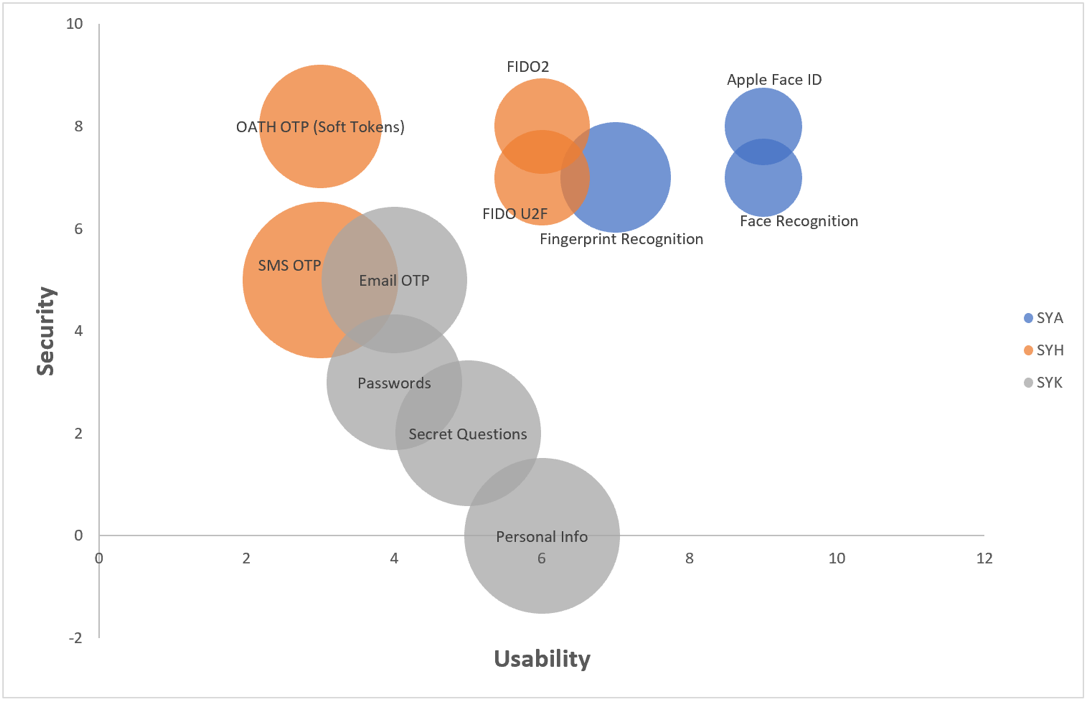
\includegraphics[width=1\linewidth]{imgs/wyk1.png}
	\caption{Porównanie metod uwierzytelniania}
	\label{fig:metody-uwierzytelniania-porownanie}
\end{figure}


\section{Sztuczne Sieci Neuronowe}
\section{Wykorzystywane narzędzia}
\subsection{Angular}
% https://vavatech.pl/technologie/frameworki/angular
% https://www.plukasiewicz.net/Angular/Angular8DataBinding

Angular jest frameworkiem do tworzenia stron internetowych typu SPA (ang. Single Page Application). Jest opracowany i rozwijany przez firmę Google. 
\paragraph{Architektura}\mbox{}\\
Podstawowym elementem architektury aplikacji Angularowych są komponenty które grupuje się, zazwyczaj ze względu na funkcjonalność, w modułach. Dzięki takiemu podejściu aplikacje są łatwo saklowalne a sama architektura przejżysta. Należy pamiętać, że wymagany jest przynajmniej jeden moduł główny w którym definiowane są najważniejsze zależności i komponenty.

\paragraph{Komponenty}\mbox{}\\
Są to pojedyncze bloki, z których zbudowana jest aplikacja napisana przy użyciu tego frameworka. Na komponent składa się zazwyczaj zestaw 3 plików składowych, z których każdy pełni określoną rolę:
\begin{itemize}
  \item Plik logiki (*.ts) --- zawierający logikę danego komponentu, w tym metody, zmienne oraz obsługę zdarzeń. W tym pliku możliwy jest import dodatkowych bibliotek lub funkcji aby rozszerzyć funkcjonalność i działanie danego komponentu 
  \item Plik szablonu (*.html) --- definiuje strukturę i wygląd komponentu. Oprócz podstawowych znaczników HTML można umieszczać w nim specjalne wbudowane lub własne dyrektywy dzięki którym można rozszerzyć funkcjonalność komponentu.
  \item Plik szablonu styli (*.css) --- służy do definicji wyglądu i formatowania komponentu zgodnie z przyjętymi założeniami projektowymi aby tworzyć estetyczne i interaktywne komponenty
\end{itemize}

\paragraph{Dekoratory klas}\mbox{}\\
Służą one do modyfikacji podstawowych klas do elementów architektury Angulara. Oprócz dekoratora \emph{@Component}, służącego do definiowania komponentu, można wyróżnić dwa dodatkowe, najbardziej podstawowe dekoratory:
\begin{itemize}
  \item @NgModule --- służy do definiowania modułu angularowego, który służy do grupowania elementów w logiczne jednostki. W modułach można między innymi deklarować komponenty, wchodzące w skład danego modułu, importować zewnętrzne moduły, aby rozszerzyć funkcjonalność oraz eksportować takie elementy, które mogą zostać wykorzystane w innym module.
  \item @Injectable --- pozwala tworzyć serwisy, usługi które mogą służyć do udostępnienia wspólnej funkcjonalności między komponentami lub częściami aplikacji
\end{itemize}

\paragraph{Powiązanie danych}\mbox{}\\
Jest to podstawowa koncepcja, która służy do komunikacji danych w komponencie i łączenia danych z widokiem. Angular oferuje wiązania jedno oraz dwukierunkowe. Wyróżnia się cztery typy wiązań:
\begin{itemize}
  \item String Interpolation --- jednokierunkowe wiązanie, którego zadaniem jest wyświetlanie danych w widoku. 
  \item Property Binding --- jednokierunkowe wiązanie, pozwala na wiązanie właściwości znaczników HTML z danymi komponentu.
  \item Event Binding --- jednokierunkowe wiązanie, które pozwala na obsługę zdarzeń wywołanych po interacji z elementami widoku
  \item Two-way binding --- dwukierunkowe wiązanie, pozwalające na wyświetlanie danych z komponentu i edycję takich danych przez użytkownika 
\end{itemize}

\begin{figure}[ht]
	\centering
		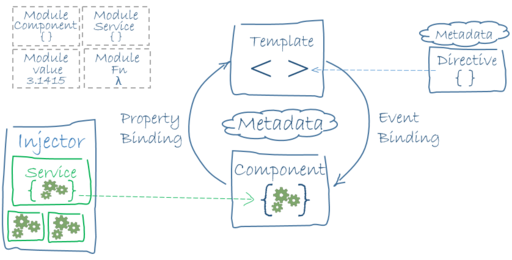
\includegraphics[width=0.6\linewidth]{imgs/ang-diag-1.png}
	\caption{Diagram powiązania elementów Angulara}
	\label{fig:wiazanie-elementow-angular}
\end{figure}

\subsection{NestJS}
% https://geek.justjoin.it/nestjs-czym-jest-jakie-ma-funkcje-jakie-sa-wady-i-zalety-tego-frameworka/
Nest JS jest frameworkiem opartym o platformę Node.JS, służącym do tworzenia aplikacji po stronie backendu z wykorzystaniem języka TypeScript. Wykorzystuje architekturę modułową, podobną do tej wykorzystywanej we frameworku Angular, dzięki czemu możliwe jest tworzenie skalowanych i wydajnych aplikacji.
\paragraph{Modułowość}\mbox{}\\
Podobnie jak we frameworku Angular, modułowość służy do grupowania elementów w logiczne jednostki. W modułach definiowane są poszczególne elementy składowe aplikacji oraz potrzebne, do poprawnego funkcjonowania, zależności.

\paragraph{Kontrolery i serwisy}\mbox{}\\
Serwisy, podobnie jak komponenty w Angularze, są pojedynczymi elementami w których zawarta jest logika biznesowa związana z konkretną funkcjonalnością. Dodatkowo w serwisach często wykonywane są podstawowe operacje CRUD bezpośrednio na modelach bazy danych. \\
Kontrolery służą do komunikacji między aplikacją kliencką a logiką biznesową z wykorzystaniem protokołu HTTP oraz podstawowych metod GET, POST, PUT, PATCH oraz DELETE.

\paragraph{Wzorce projektowe}\mbox{}\\
Nest.JS jest opracowany tak, aby można było korzystać z popularnych wzorców projektowych, takich jak wstrzykiwanie zależności oraz odwrócenie kontroli, co pozwala zapewnić lepszą strukturę i architekturę aplikacji.

\paragraph{NPM}\mbox{}\\
Z tego powodu, że Nest.JS oparty jest o platformę Node.JS to wspiera repozytorium NPM. Dzięki temu podstawowe funkcjonalności można rozszerzać o dodatkowe i często wykorzystywane biblioteki tworząc zaawansowane, biznesowe aplikacje backendowe.

\begin{figure}[ht]
	\centering
		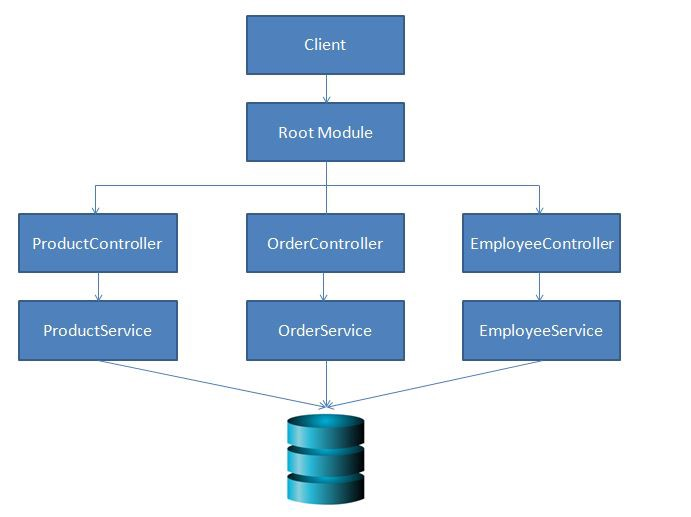
\includegraphics[width=0.6\linewidth]{imgs/nest-diag.jpeg}
	\caption{Schemat uproszczonej architektury aplikacji}
	\label{fig:nest-uproszczona-architektura}
\end{figure}

\subsection{Python}
W kręgach entuzajstów uczenia maszynowego oraz sztucznych sieci neuronowych można zauważyć dużą popularność przy wykorzystaniu języka Python do implementacji takich rozwiązań. Sam język jest wysokopoziomowym, interpretowalnym językiem programowania ogólnego przeznaczenia. Dzięki swojej czytelnej, prostej składni jest wykorzystywany w wielu dziedzinach, w tym algorytmach sztucznej inteligencji.

\paragraph{Składnia}\mbox{}\\
W przeciwieństwie do sporej liczby języków programowania, Python wykorzystuje prostą, przejrzystą składnię opartą na wcięciach. Między innymi przez swoją składnię jest wybierany jako pierwszy język do nauki programowania

\paragraph{Dynamiczne typowanie}\mbox{}\\
Programując przy użyciu tego języka można zauważyć, że zmienne lub metody nie muszą mieć określonego typu. W przeciwieństwie do innych języków, typ danych określany jest dynamicznie w trakcie wykonywania programu, dzięki czemu zyskał on dużą popularność w zakresie data science.

\paragraph{Biblioteki}\mbox{}\\
Jedną z zalet Pythona jest obszerna biblioteka standardowa, która zapewnia dostęp do różnych klas oraz funkcji. Dzięki temu na start użytkownik otrzymuje bardzo rozbudowane narzędzie programistyczne, które nadaje się do różnych zastosowań. Warto również zwrócić uwagę na rozbudowaną społeczność tego języka, która tworzy i udostępnia własne biblioteki, a część z nich stała się już obecnie standardem. Dla przykładu wiele rozwiązań z zakresu uczenia maszynowego opiera się o popularne biblioteki pokroju NumPY lub MatplotLib które ułatwiają i usprawniają pracę na danych tabelarycznych oraz pomagają wizualizować dane w różny sposób.

\subsection{MongoDB}
%https://appmaster.io/pl/blog/czym-jest-mongodb
Bazy danych są bezpośrednio związane z rozwiązaniami informatycznymi już od wielu lat. Dawniej obowiązującym standardem były relacyjne bazy jak na przykład MySQL, które były znane z powiązań relacyjnych między tabelami w bazie. Obecnie można zauważyć wzorst popularności rozwiąząń nierelacyjnych baz danych w tym MongoDB.
Jest to baza danych, w której obiekty, dane przechowywane są w postaci dokumentów, strukturą zbliżoną do obiektów JSON. Charakterystyczne dla takich baz jest brak ściśle zdefiniowanej struktury obiektów, przez co dane wchodzące w skład kolekcji moża różnić się strukturą między sobą.
Dodatkowo MongoDB jest znane z bardzo dobrej skalowalności, zarówno poziomej jak i pionowej, obsługi bardzo dużej ilości danych oraz wsparcia dla wielu języków programowania dzięki czemu bardzo łatwo jest wykorzystać tą bazę w projekcie. 

\subsection{RabbitMQ}
% https://czterytygodnie.pl/rabbitmq/wprowadzenie-do-kolejkowania-rabbitmq.html
Mówiąc o systemach mikroserwisowych warto wspomnieć o mechanizmach, które pozwalają na komunikację między poszczególnymi serwisami. Jest wiele różnych narzędzi wspierających taki proces a jednym z nich jest wykorzystanie brokera wiadomości.
Jednym z popularniejszych systemów oferujących takie rozwiązanie jest RabbitMQ. Pozwala na wysyłanie i odbieranie wiadomości przy wykorzystaniu kanałów oraz kolejek wiadomości. Wieloplatrofmowość oraz wsparcie dla wielu popularnych języków programowania sprawia, że omawiane narzędzie jest bardzo często wykorzystywane do łączenia ze sobą mikroserwisów, nawet tych napisanych przy wykorzystaniu różnych języków programwnia. Dzięki swojej skalowalności i elastyczności, RabbitMQ zyskuje popularność w wielu systemach informatycznych.


\subsection{Docker}
% https://sii.pl/blog/docker-dla-programistow-co-to-jest/?category=development-na-twardo&tag=devops,docker,kontener
Badjąc statystyki opisujące które technologie, zdaniem programistów, są najbardziej pożądane można zauważyć, że oprócz znajomości systemu kontroli wersji (git) na takim samym poziomie jest znajomość Dockera. W dobie rozwiązań chmurowych, mikroserwisowych wirtualizacja środowisk, systemów informatycznych jest niezwykle ważnym tematem ponieważ zapewnia jednolite działanie systemu bez względu na platformę na której jest uruchamiany. Dzięki solidnej realizacji tego zadania Docker zyskał niezwykłą popularność na przełomie kilku ostatnich lat 
Najprościej mówiąc, Docker jest narzędziem do wirtualizacji środowisk programistycznych, wykonawczych, które oferuje tworzenie niezależnych od siebie kontenerów. Kontener jest lekkim, samodzielnym oraz wykonywalnym pakietem oprogramowania który zawiera wszystko, co niezbędne aby dany serwis lub usługa została uruchomiona.
\subsection{Face Recognition}
% https://medium.com/@ageitgey/machine-learning-is-fun-part-4-modern-face-recognition-with-deep-learning-c3cffc121d78
W wielu serwisach i aplikacjach internetowych, oferujących publikowanie zdjęć użytkowników, wykorzystuje algorytmy do detekcji twarzy, a czasem nawet i rozpoznawanie twarzy użytkowników na zdjęciach. Do jeszcze nie tak dawna temu, narzędzia oferujące tego typu rozwiązania nie były dostępne dla początkujących programistów, a przynajmniej nie za darmo. Chcąc zaimplementować mechanizm detekcji lub rozpoznawania twarzy należało samemu opracować oraz wytrenować model sieci neuronowej. Jednak proces ten nie należy do najłatwiejszych i wymaga odpowiedniej wiedzy i doświadczenia do tego, aby stworzyć model, który ma predykcję na dobrym poziomie i \textbf{można mu ufać (#CHANGE)}.
Od niedawna dostępna jest otwartoźródłowa biblioteka dla języka Python, oferująca proces detekcji i rozpoznawaia twarzy na bardzo dobrym poziomie z dokładnością do 98\%.\\

\subsection{Xception}